\documentclass[]{article}
\usepackage{graphicx}
\graphicspath{{figures/}}
%opening
\title{RL exercise 07 }
\author{Mengnan Wang}

\begin{document}

\maketitle

\section{Normalized gradient}
\paragraph{}Gradient ascent with fixed step-size $alpha=0.5$, shown in figure \ref{fig:fix-alpha}.
\begin{figure}[!htb]
	\centering
	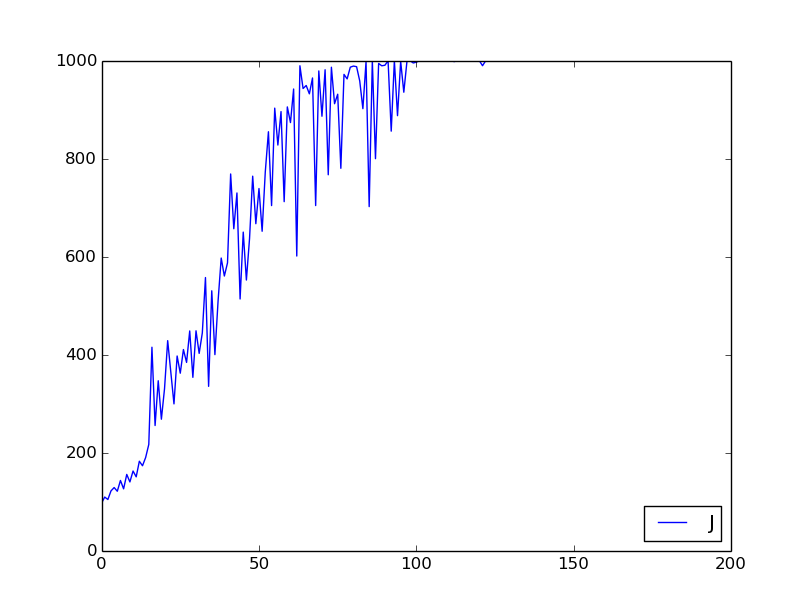
\includegraphics[width=\linewidth]{FD.png}
	\caption{\label{fig:fix-alpha}Fixed step size $alpha=0.5$}
	\end{figure}
\section{Heuristic step-size}
\paragraph{}I first choose line search and wolfe condition to select step-size. While the result showed that wolfe condition was prone to 'jump' into local maximum but it was very stable inside local maximum, figure \ref{fig:wolfe}. 
\paragraph{}Using decreasing step-size $\alpha_t=\frac{10}{t}$, the parameter converges quickly but it will fluctuate for a while, figure \ref{fig:decrease}.
\paragraph{}So i combine wolfe condition with $\alpha_t=\frac{10}{t}$. Since the maximal time step of each episode is 1000, the best expect reward should be 1000. With this prior knowledge, i first use $\alpha_t=\frac{10}{t}$ to choose step-size. After the expect reward is larger than 800. I switch to line search and wolfe condition for choosing step-size. The result shows that after expect reward is larger than 800, the parameter quickly converges to global optimum and stick to it, figure \ref{fig:wolfe+decrease}. 
\begin{figure}
	\centering
	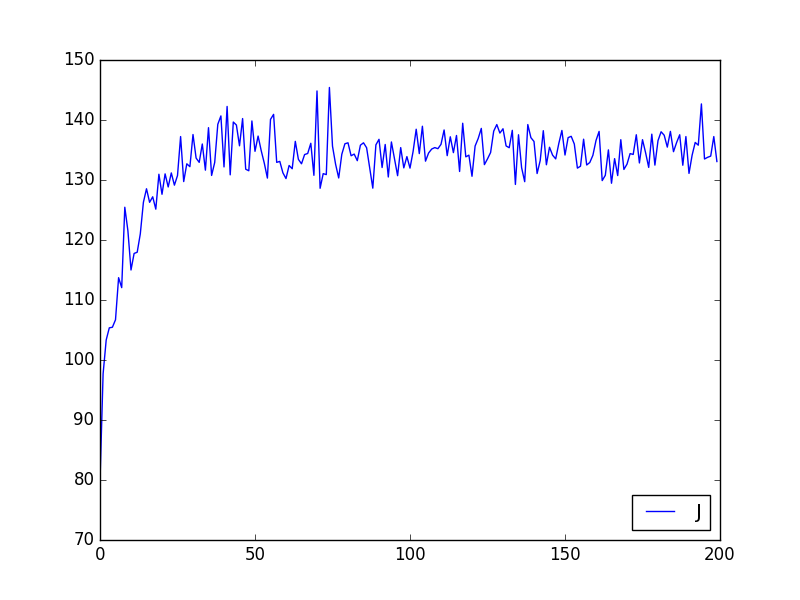
\includegraphics[width=\linewidth]{wolfe.png}
	\caption{\label{fig:wolfe}Wolfe condition and line search}
\end{figure}
\begin{figure}
	\centering
	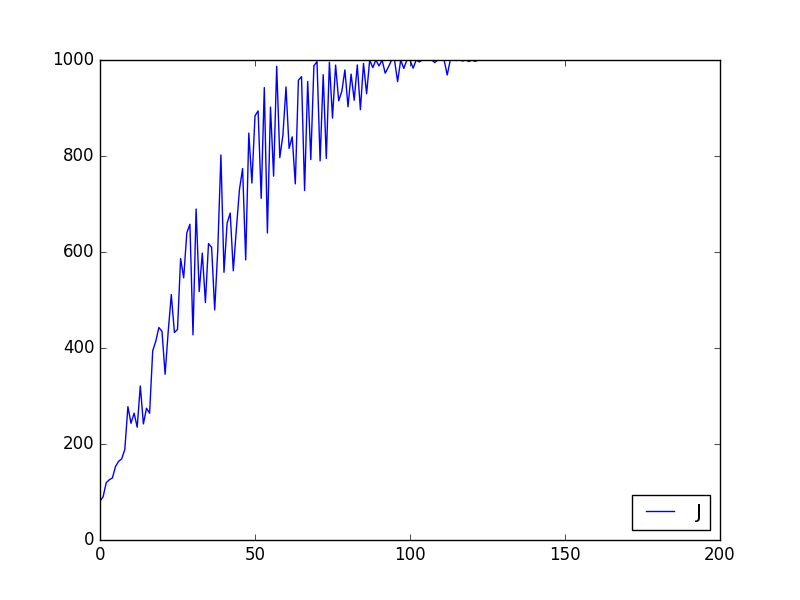
\includegraphics[width=\linewidth]{decrease.png}
	\caption{\label{fig:decrease}Decreasing step-size$\alpha_t=\frac{10}{t}$}
\end{figure}
\begin{figure}
	\centering
	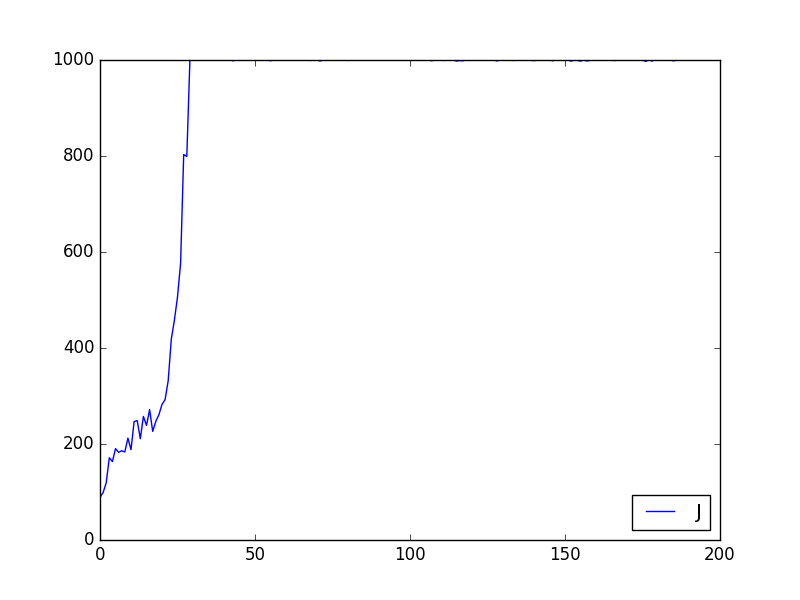
\includegraphics[width=\linewidth]{wolfe+decrease.png}
	\caption{\label{fig:wolfe+decrease}Combined step-size}
\end{figure}

\section{Adaptive step-size}
\paragraph{}I only run adaptive step-size for 20 iteration, since it converges very fast, figure \ref{fig:adp-step-size}.
\begin{figure}
	\centering
	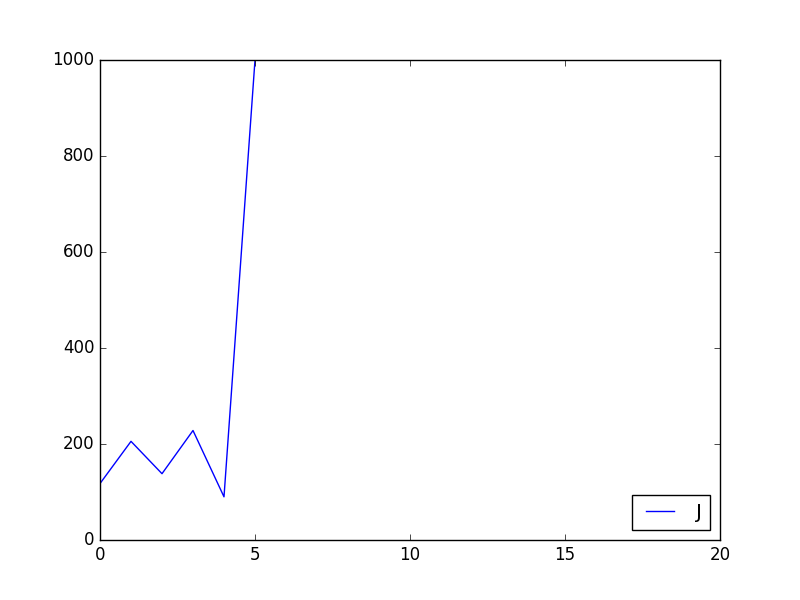
\includegraphics[width=\linewidth]{FD_Rprop.png}
	\caption{\label{fig:adp-step-size}Adaptive step-size}
\end{figure}

\end{document}
